
% =========================================================================
\section{Method}
\label{sec:method}

In this section, we present \CropCode{}, a multimodal framework for recovering
procedural plant representations from incomplete sensor observations. We first
formulate the reconstruction task and describe the procedural data generation
process. Next, we introduce the token representations and masked pretraining
objective. Finally, we describe the teacher--student training strategy for
single-sensor inference and the protocol used to evaluate transfer to field
observations. An overview of the framework is shown in Fig.~\ref{fig:arch}.


% ---- FIG 2 (architecture, full width): four token streams entering a
% shared encoder (RGB patches / depth patches / PC groups / xVal param
% tokens), Dirichlet mask sampler on top, four decoders out; a second
% panel showing teacher (all streams) -> distill -> student (one stream).
\begin{figure*}[t]
  \centering
  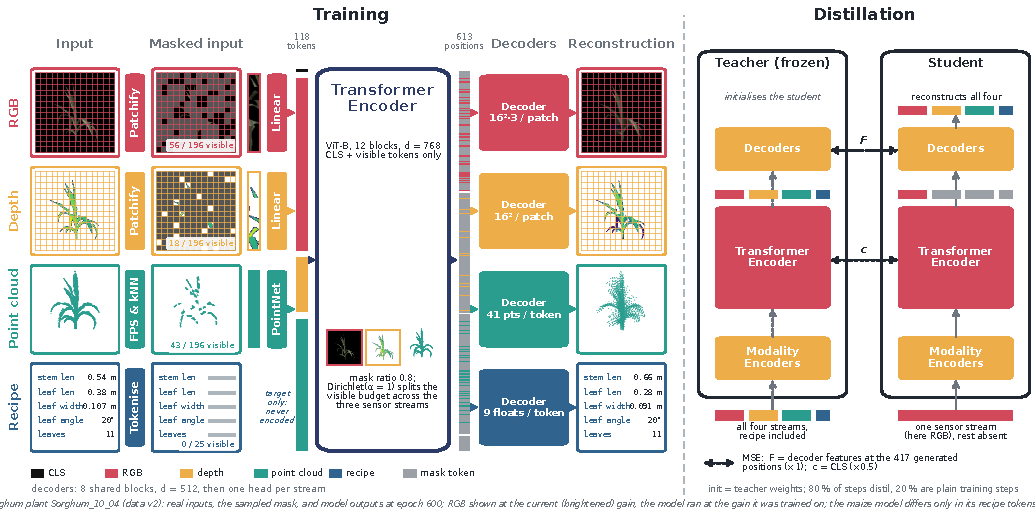
\includegraphics[width=\linewidth]{Figures/fig_architecture.pdf}
  \caption{\textbf{\method{} overview.} (a) Four token streams enter a
  shared encoder under a Dirichlet masking budget; modality-specific
  decoders reconstruct all streams. During pretraining the parameter
  stream is both masked input and decoder target; its role is ablated in
  Sec.~\ref{sec:exp-params}. (b) The full-modality
  teacher is distilled into single-sensor students for deployment.}
  \label{fig:arch}
\end{figure*}

\subsection{Problem formulation}
\label{sec:method-form}
% Talking points:
% - A plant is a program: theta in R^d (plant-level + per-leaf fields;
%   d ~ \todo{X} for maize, \todo{Y} for sorghum), generator G(theta) ->
%   mesh -> any sensor rendering.
% - Observation: O = any nonempty subset of {I_rgb, I_depth, P_partial},
%   degraded by view sparsity, sensor noise, and ROW OCCLUSION (neighbor
%   points inside the target's region, bent-leaf contact geometry).
% - Task: a single amortized f(O) -> (theta_hat, I_rgb, I_depth, P_full):
%   procedural parameters PLUS completed modalities, one forward pass.
% - State the well-posedness argument: slender+occluded geometry is
%   underdetermined; G's parameterization is the prior that closes it.
\todo{3 short paragraphs from the bullets}

Let $G$ denote a procedural generator that maps a parameter vector
$\theta\in\R^{d_\theta}$ to a plant mesh $G(\theta)$. The parameters describe
plant-level structure, including stem and panicle geometry, together with
leaf-level attributes such as insertion height, length, roll, branching angle,
and blade width. We consider three sensor modalities,
$\mathcal{M}=\{\mathrm{rgb},\mathrm{d},\mathrm{pc}\}$, corresponding to an RGB
image, a depth frame, and a point cloud. In field conditions, only a subset
$S\subseteq\mathcal{M}$ may be available, and each observation may contain
partial geometry or occlusion from neighboring plants. Our objective is to
recover the underlying procedural representation from these observations.

We formulate this task as feed-forward prediction:
\begin{equation}
  f_\phi\!\left(\{x^m:m\in S\}\right)
  = \left(\hat\theta,\{\hat x^m:m\in\mathcal{M}\}\right),
  \label{eq:procedural-inverse}
\end{equation}
where $\phi$ denotes the network parameters, $\hat\theta$ is the predicted
plant description, and $\hat x^m$ denotes the reconstructed sensor modalities.
The procedural output $G(\hat\theta)$ supports geometric reconstruction and
trait analysis within the same representation. Unlike per-instance fitting
of a procedural model to a scan~\cite{hadadi2026vlmmaize}, this formulation
learns a shared inverse mapping that is applied to each new observation in a
single forward pass.

The procedural generator provides both the training observations and their
exact parameter targets. This allows us to supervise parameter recovery
without manually annotating each synthetic plant. At deployment, however,
$\theta$ is unknown and must be inferred exclusively from sensor input. We
therefore distinguish its role as a reconstruction target from its possible
use as privileged input during training. The visibility of the parameter
stream is controlled separately, allowing us to study this distinction while
keeping the sensor-token budget fixed (Sec.~\ref{sec:param-stream}).



\subsection{A procedural field-data engine}
\label{sec:method-data}

\begin{table}[t]
  \centering\small
  \setlength{\tabcolsep}{3pt}
  \begin{tabular}{lcc}
    \toprule
     & Maize & Sorghum \\
    \midrule
    Plants & 15{,}000 & 15{,}000 \\
    Split (train/val/test) & \multicolumn{2}{c}{10{,}500 / 2{,}250 / 2{,}250} \\
    Views per plant & 10, random & 10, fixed rig \\
    Camera distance & fitted per plant & 2.5\,m \\
    Per-view cloud & 8{,}192 pts, visible & complete \\
    Parameter slots ($d_\theta$) & $14+14\times28$ & $9+5\times24$ \\
    Leaf count range & \todo{3--22} & 4--35 \\
    Plant height & 0.62--1.44\,m & stem 0.19--1.74\,m \\
    Rows $\times$ orientations & $15{,}000\times10$ & $15{,}000\times10$ \\
    Row camera & level, 1.0\,m & level, 2.5\,m \\
    Row cloud in / target & \multicolumn{2}{c}{24{,}576 / 8{,}192 pts} \\
    Real-field split & \todo{MaizeField3D} & \todo{TBD} \\
    \bottomrule
  \end{tabular}
  \caption{\FieldProc{} dataset configuration. The parameter dimension
  includes plant-level attributes and a fixed number of leaf slots. Every
  row has one main plant from the split and two neighbours at a 0.15\,m
  stem spacing, widened only when the contact solver needs it
  (Supp.~\ref{app:data}). \todo{Confirm the maize leaf-count range and the
  real-data splits~\cite{maizefield3d2025}.}}
  \label{tab:fieldproc}
\end{table}

\paragraph{Procedural generation.}
We construct \FieldProc{} using species-specific generators for maize and
sorghum, 15{,}000 plants each. Plant $i$ is generated with random seed $i$ and
is paired with its exact procedural parameters. Maize traits are drawn from
Gaussians (e.g.\ height $0.83\pm0.10$\,m, leaf count $12.4\pm2.6$, leaf angle
$44^\circ\pm10^\circ$) coupled through four latent traits (vigour, slenderness,
posture, texture), with canopy-position curves and per-leaf jitter; the plants
are 0.62--1.44\,m tall. Sorghum plants come from the EvoEngine sorghum
generator, which draws the heading, stem tilt, leaf count and internode length
per plant and evaluates per-leaf curves for insertion point, length, width,
roll (alternating sides), branching angle and bending; they carry 4--35 leaves
(mean 19.5) on stems of 0.19--1.74\,m. The populations therefore span
continuous variations in morphology rather than discrete genotype classes,
and we evaluate phenotype representations through regression. The generators
also differ in their trait dependencies. In sorghum, stem length is the
internode length times the leaf count, so it is strongly coupled to leaf
count ($\text{stem length}=0.05\,n_{\text{leaves}}-0.001$, $R^2=0.988$),
whereas this association is weak in maize ($r=0.20$). We therefore evaluate
both species to examine whether the observed behavior extends beyond a single
generator's correlations.

\paragraph{Isolated-plant observations.}
For each plant, we render ten views with \texttt{pyrender} at $1024\times1024$
and a $40^\circ$ vertical field of view, each with an RGB image, a depth image
stored losslessly as a packed 32-bit value, and the camera pose. Three fixed
directional lights are aimed at the plant's bounding-box centre. Images are
rendered on a grey background; in the final release it is made transparent
and composited over black. The
two species are captured differently. Sorghum views follow one fixed
Fibonacci-sphere rig at 2.5\,m, five directions above and five below the
horizon (elevations $-64^\circ$ to $+64^\circ$), so every plant is seen from
the same ten directions, and the per-view cloud is the complete,
occlusion-free plant cloud expressed in the camera frame. Maize views are ten
directions drawn uniformly on the sphere per plant, at a distance fitted to
the plant's bounding box, with an extra light at the camera; the per-view
cloud is 8{,}192 points back-projected from that view's depth image, so it
holds only the surface the camera sees. At 2.5\,m the lens covers about
1.8\,m of height, so the top or base of the tallest sorghum plants can fall
outside the frame.

\paragraph{Row observations.}
The row sets place each plant of a split, as the \emph{main} plant, between two
neighbours from the same split (one row per plant), with 0.15\,m between stem
bases. Each row is rendered at ten orientations: the main plant is turned
about its stem by $0^\circ,10^\circ,\dots,90^\circ$ and each neighbour by the
same angle plus a uniform offset in $\pm15^\circ$; sorghum neighbours are also
tilted so their stems run parallel to the main stem. Before rendering, a
contact solver makes the three plants free of intersections while keeping
them close to their grown shapes: each leaf blade is a chain of 8\,cm
segments whose joints bend along circular arcs, so blades stay smooth, keep
their length and stay attached, while stems, sheaths and tassels stay rigid.
A leaf that would cross another plant bends by the smallest clearing angle at
the joint before the contact; neighbours give way first, and a main-plant leaf
bends only where a neighbour cannot move. Contacts are decided by exact
triangle--triangle tests, so leaves may touch but never intersect. When no
layout exists under the bend limits, the limits are loosened in stages and
then the spacing is widened; in maize, 76--79\,\% of orientations are solved at
0.15\,m and none needs more than 0.33\,m. A rover camera, level and aimed at
the main plant's bounding-box centre from 1.0\,m (maize) or 2.5\,m (sorghum),
takes one shot per orientation, rendered twice: the input with all three
plants (RGBA, depth, and a 24{,}576-point cloud of every visible plant) and the
ground truth with the main plant alone, in its bent shape, from the same
camera (8{,}192 points). The parameter record describes the grown plant, so
the target geometry departs from it only where the solver had to bend a
main-plant leaf.
Occlusion is measured per shot from the two depth maps (maize, 120 train
rows): the fraction of the main plant's own pixels hidden behind a neighbour is
9\,\% on average, 13\,\% at $0^\circ$, where the generator's single leaf plane
lies along the row, falling to 1\,\% at $90^\circ$ (90th percentile 17\,\%),
and the neighbours supply 59--68\,\% of the plant pixels in the frame and two
thirds of the input cloud. \todo{Same measures for the sorghum rows.}

\paragraph{Data partitioning.}
We partition plants into training, validation, and test sets in a 70/15/15
ratio by plant, so all views and rows of a main plant fall in one split, and
we bias the held-out sets toward unusual morphologies. For maize, each plant is
scored by its Mahalanobis distance~\cite{mahalanobis2018generalized} from the
median over 19 robustly standardized parameter features, and the most extreme
plants are dealt alternately to test and validation, a pure tail split. For
sorghum, the extremeness is the Mahalanobis distance from the mean over six
features (leaf count, stem length, mean and maximum leaf length, mean and
standard deviation of leaf roll), and the probability of being held out rises
steadily with its rank, from 0.3\,\% in the least extreme 5\,\% of plants to
70\,\% in the most extreme 5\,\%; validation and test share one distribution.
\todo{The sorghum selection rule is inferred from the released assignment;
confirm it against the script that wrote it.}
We report errors in native trait units alongside $R^2$, since the latter
depends on the target distribution of each split. In the ablations, an epoch
samples one view per training plant, with identical view draws across compared
models. Data-scaling experiments use nested subsets of plants, each retaining
all ten available views, and match the number of optimizer updates.
% Original split diagnostic: median extremeness is 2.03 on train and 2.76 on
% validation/test. Retain in the dataset supplement; define rank scaling.




% - Two generators, two species: FloraForge maize (BTx99 phenotype,
%   rebuildable-from-file parameters) \citep{floraforge2026}; EvoEngine
%   sorghum. Hidden-trait correlation structure (vigor, slenderness,
%   posture, texture).
% - Row simulation: neighbors at d=0.40m, contact-resolved leaf bending
%   (no interpenetration, arcs preserve length), rotation about stem.
% - Capture model: 10 views/plant, 1024^2 RGB + metric depth, 8,192-pt
%   per-view camera-frame clouds, 60K-pt whole-plant GT; crop-box inputs
%   retain ~1/3 contaminating neighbor points.
% - Scale: \todo{10K-100K} plants/species; 70/15/15 split by plant.
% - BIOLOGICALLY CONSTRAINED SAMPLING: correlated developmental traits
%   (height, leaf count, internode spacing, insertion locations) sampled
%   jointly from allometrically constrained distributions WITH NOISE —
%   correlated but never deterministic (target the maize regime,
%   r~0.2 height/leaf-count, NOT sorghum's r=0.994 coupling, which
%   collapses trait evaluation to rank 2). Report conditional spreads.
%   Estimate the allometry from measured maize data where possible.
% - PARAMETER GROUPING: plant-level/developmental (height, leaf count,
%   stem diameter, internodes, insertion locations) vs organ-level/shape
%   (length, width, insertion angle, azimuth, droop, curvature, twist).
%   Headline evaluation traits: height, leaf count, leaf angle, length,
%   width, azimuth; waviness/spline fields stay in the representation
%   but not in headline metrics.
% - PAIRED OBSERVATIONS: every plant rendered BOTH isolated AND inserted
%   into a row (same morphology, harder observation); row spacing swept
%   \todo{0.15-0.70 m}; per-sample occlusion severity recorded
%   continuously (visible pixel fraction, visible 3D-point fraction,
%   neighbor contamination, hidden-leaf fraction).
% - CAMERA PROTOCOL: explicit, evidence-based axes — elevation ladder
%   (the documented difficulty axis) and azimuth relative to the leaf
%   plane (distichous maize); small schematic figure.
% - BACKGROUND / SENSOR MODEL: \todo{if the real acquisition commits to
%   strobe + short exposure, frame the dark background as a deliberate
%   sim-to-real co-design and add the black-vs-randomized-background
%   ablation evaluated on real strobe images; current captures use 0.5
%   grey — verify acquisition plan before adopting}.
% - Close with: exact parameter GT for every sample — the supervision no
%   real capture can provide.
% \begin{table}[h]\centering\small
% \begin{tabular}{lcc}
% \toprule
%  & Maize & Sorghum \\
% \midrule
% Plants                     & \todo{N}        & \todo{N} \\
% Views / plant              & 10              & 10 \\
% Parameters / plant         & \todo{d}        & \todo{d} \\
% Leaf count range           & 3--22           & 11--27 \\
% Occluded-row variants      & \todo{...}      & \todo{...} \\
% Neighbor points in crop   & \todo{$\sim$30\%} & \todo{...} \\
% \bottomrule
% \end{tabular}
% \caption{\dataset{} at a glance. \todo{finalize; add diversity axes
% (phenotypes / generator configs / growth stages) and real-data eval row
% (MaizeField3D scans + pipeline GT \citep{maizefield3d2025,
% hadadi2026vlmmaize})}}
% \label{tab:data}
% \end{table}



% ---- The "only row with all checkmarks" exhibit. Verified by the lit
% review: no existing dataset combines these properties.
\begin{table*}[h]\centering\small
\begin{tabular}{lcccccc}
\toprule
 & Real & Slender & Row occl. & RGB+D+PC & Proc.\ GT & Scale \\
\midrule
PCN / ShapeNet-55~\citep{yuan2018pcn,yu2021pointr}
          & \xmark & \xmark & \xmark & \xmark & \xmark & 55K \\
Pheno4D~\citep{schunck2021pheno4d}
          & \cmark & \cmark & \xmark & \xmark & \xmark & 84 \\
Crops3D~\citep{crops3d2024}
          & \cmark & \cmark & \xmark & \xmark & \xmark & \todo{} \\
MaizeField3D~\citep{maizefield3d2025}
          & \cmark & \cmark & \xmark & \xmark & (\cmark) & 1K \\
\dataset{} (ours)
          & \cmark$^{\dagger}$ & \cmark & \cmark & \cmark & \cmark
          & \todo{N} \\
\bottomrule
\end{tabular}
\caption{Dataset comparison. Proc.\ GT: exact generative parameters per
plant; (\cmark): fitted post hoc rather than exact.
$^{\dagger}$real-field evaluation split; training data is procedural.
\todo{verify Crops3D scale; consider adding A-Occ-Plant's data if
released}}
\label{tab:datacompare}
\end{table*}

\subsection{Four-stream masked pretraining}
\label{sec:method-pretrain}
% - Tokenization: ViT patches (RGB, depth), FPS groups (PC, 196 tokens),
%   xVal-style continuous number tokens for parameters
%   \citep{golkar2023xval} — one token per scalar, plant row + per-leaf rows.
% - Masking: Dirichlet split of a 0.80 budget across visible streams,
%   min per-modality ratio 0.25 — every subset becomes a training task.
% - Losses: MSE (RGB, depth), Chamfer/QAL (PC), param regression loss;
%   per-head weights \todo{values}.
% - As run: the headline model and teacher encode the parameter stream
%   (shared Dirichlet budget); Sec.~\ref{sec:exp-params} ablates this.
\todo{2-3 paragraphs}

\paragraph{Token representations and architecture.}
Our architecture builds on EmbodiedMAE~\cite{dong2025embodiedmae}, extending
its sensor streams with a structured parameter representation. RGB and depth
are each represented by 196 patch tokens on a $14\times14$ grid, with fixed
2-D sine--cosine positional embeddings. Following
Point-MAE~\cite{pang2022pointmae}, we select 196 point-cloud centers through
farthest-point sampling and group their 32 nearest neighbors. A local
PointNet~\cite{qi2017pointnet} embeds each group using coordinates relative
to its center. The parameter stream consists of $1+K$ tokens: one for
plant-level attributes and $K$ for individual leaves, with $K=24$ for sorghum
and $K=28$ for maize. Each attribute is affinely normalized to $[0,1]$ and
linearly projected, retaining continuous numerical values rather than text
tokens, in the spirit of xVal~\cite{golkar2023xval}. A validity mask identifies
padded leaf slots. Learned modality embeddings distinguish the streams, and a
CLS token is prepended to the visible sequence. A 12-block encoder of width
768 processes this sequence, followed by an 8-block decoder of width 512.
The decoder restores a fixed ordering of all $L=588+(1+K)$ token positions
using mask tokens for missing inputs. Linear heads reconstruct RGB and depth
patches, a FoldingNet-style head generates 41 points per point-cloud token,
and an MLP predicts the procedural parameters.
Plants with more than $K$ leaves keep their first $K$ leaf tokens.
\todo{Define inference-time leaf presence; report the share of sorghum plants
above $K=24$.}

\paragraph{Modality masking.}
We use a total mask ratio of $\rho=0.80$ over all four streams, giving a
visible budget
\begin{equation}
  V=\left\lfloor(1-\rho)\sum_{m\in\mathcal{M}}L_m\right\rfloor,
  \label{eq:visible-budget}
\end{equation}
which is 122 tokens for sorghum ($L=613$) and 123 for maize ($L=617$). At
each training step, a sample from $\mathrm{Dirichlet}(\mathbf{1})$ allocates
this budget across the four streams, the parameter stream included. Integer
allocations preserve the exact budget, retain at least one token per stream,
and mask at least 25\% of each stream. Token counts are shared across a batch,
while visible positions are sampled independently for each example. The
procedural parameters are therefore both an encoder input and a decoder
target in the headline model: because the parameter stream is short, it is on
average $\sim$58\% visible, while the three sensor streams together keep about
107 of their 588 tokens.

For the controlled ablations of Sec.~\ref{sec:param-stream}, the parameter
stream can instead be taken out of the shared budget and masked at its own
ratio $\rho_\theta$:
\begin{equation}
 V_\theta=
 \begin{cases}
  0, & \rho_\theta=1,\\
  \max\!\left(1,\left\lfloor(1+K)(1-\rho_\theta)\right\rfloor\right),
    & 0\leq\rho_\theta<1,
 \end{cases}
 \label{eq:parameter-visibility}
\end{equation}
with the Dirichlet budget then allocated over the three sensor streams alone
($V=117$). This keeps the sensor masks identical across matched three- and
four-stream arms under the same seed. $\rho_\theta=1$ makes the parameters a
reconstruction target only, never an encoder input. Parameters are never an
input at deployment, where only sensor streams are available.
% Original shared-budget diagnostic: about 59% parameter visibility versus
% 18% sensor visibility, compared with 20% in the sensor-only allocation.
% Keep this empirical finding in the token-budget ablation.


\paragraph{Reconstruction objective.}
We jointly optimize the four reconstruction terms:
\begin{equation}
  \mathcal{L}_{\mathrm{rec}}=
  \ell_{\mathrm{rgb}}+\ell_{\mathrm{d}}+
  \ell_{\mathrm{pc}}+5\ell_\theta.
  \label{eq:reconstruction-loss}
\end{equation}
The RGB loss is MSE on patch-normalized targets~\cite{he2022mae}, while the
depth loss is MSE after per-image min--max normalization. Both are evaluated
at masked positions during pretraining. The parameter loss is Smooth-L1 over
masked, valid parameter tokens. For point clouds, the loss compares the full
predicted set $\hat P$ with the target set $P$. Motivated by the limitations of
nearest-neighbor geometry objectives~\cite{wu2021dcd,song2026structural}, we
use a sigmoid-weighted Chamfer objective:
\begin{equation}
 \begin{split}
  \ell_{\mathrm{pc}}={}&
  \frac{1}{|\hat P|}\sum_{p\in\hat P}w(\delta(p,P))\,\delta(p,P)\\
  &+\frac{1}{|P|}\sum_{q\in P}w(\delta(q,\hat P))\,\delta(q,\hat P),
 \end{split}
 \label{eq:point-loss}
\end{equation}
where $\delta(p,P)=\min_{q\in P}\|p-q\|_2$ and
$w(r)=\sigma(a(r-\tau))$. We set $a=100$ and $\tau=0.01$, reducing the
weight of small residuals relative to larger reconstruction errors.
% The original formula used N in both directions. Set-specific cardinalities
% above clarify the mean reduction when prediction and target sizes differ.
Both directions are averaged over their own set and then over the batch.
Clouds are centred on their centroid and scaled so the farthest point lies on
the unit sphere, so $\tau$ is relative to the plant: one percent of its radius,
about 7\,mm on a 1.4\,m plant.
Nearest-neighbour losses let many predicted points share one target point at
no cost, so the folding head can collapse a token's points into a clump and
still score well. The headline model therefore adds an optimal-transport term
that matches the two clouds as distributions, the debiased Sinkhorn
divergence~\cite{feydy2019sinkhorn},
\begin{equation}
  \ell_{\mathrm{pc}}^{\star}=\ell_{\mathrm{pc}}
  +0.5\,S_{\varepsilon}\!\left(\hat P_{1024},P_{1024}\right),
  \label{eq:point-loss-sinkhorn}
\end{equation}
with $p{=}2$ and blur $\varepsilon{=}0.02$ in the unit-sphere frame, computed
between random 1{,}024-point subsets of prediction and target that are redrawn
at every step. The term rewards coverage of the whole cloud directly, and the
subsets keep its cost matrix at $B\times1024^2$. The ablation arms of
Sec.~\ref{sec:experiments} were trained with Eq.~\eqref{eq:point-loss} alone;
the Sinkhorn term enters the headline model and the distillation.
\todo{Report the ablation of this term (E7).}
We train with AdamW, $\beta=(0.9,0.95)$, weight decay 0.05, linear warm-up,
cosine learning-rate decay, and gradient clipping at 1.0. The main schedule
uses 1,000 epochs and a global batch size of 256. Ablations instead use a
fixed budget of 197,400 optimizer steps at global batch size 32 to prevent
larger datasets from receiving more updates merely through equal-epoch
training. The main schedule visits all ten views of every training plant in
each epoch, with a peak learning rate of $6\times10^{-4}$ and a 20-epoch
warm-up. Ablations sample one view per plant per epoch, with a peak learning
rate of $1.5\times10^{-4}$ and a warm-up of 40 epochs at the full-data scale
(scaled with the epoch count when the number of plants changes).


\subsection{A full-modality teacher, single-sensor students}
\label{sec:distill}\label{sec:method-distill}

Pretraining retains visible tokens from every sensor stream. Consequently,
single-sensor inference introduces a missing-modality configuration that the
encoder has not encountered during this stage. We address this gap through
teacher--student distillation~\cite{hinton2015distillation}. The teacher is
the pretrained four-stream model, frozen: for sorghum the checkpoint with the
lowest validation loss (epoch 960 of 1{,}000), for maize the final epoch-600
checkpoint. It receives RGB, depth, point clouds, and the procedural
parameters, the same four streams it was pretrained on, so the parameters act
as privileged information that the students will not have. For sorghum every
token of every stream is visible to the teacher; for maize we retain half the
tokens of each stream to avoid the reconstruction degradation observed with
fully visible input. We assess the
teacher's reconstruction quality under the selected mask before distillation.
The teacher provides a CLS representation $c^T\in\R^{768}$ and final normalized
decoder features $F^T\in\R^{L\times512}$, where $L=613$ for sorghum and 617
for maize. The fixed decoder layout gives a direct correspondence between
teacher and student features at every output position.
% Original teacher diagnostics for experiments/supplement:
% Sorghum Chamfer: 4.8e-4 fully visible vs. 3.5e-4 at 50% visibility.
% Maize Chamfer: 0.05--0.09 fully visible vs. approximately 0.001 masked.

The student is initialized from the teacher and optimized for 100 epochs with
AdamW, a learning rate of $10^{-4}$, cosine decay, and global batch size 128.
At each step, a seeded random draw selects single-sensor training with
probability 0.8 or ordinary masked pretraining with probability 0.2. In a
single-source step, the source $s$ is cycled deterministically over all four
streams (RGB, depth, point cloud, and parameters), and only its tokens enter
the encoder; optionally, half these tokens are also
masked for regularization. The objective combines ground-truth reconstruction
with decoder- and encoder-level feature matching:
\begin{equation}
 \begin{split}
  \mathcal{L}_{\mathrm{student}}={}&\mathcal{L}_{\mathrm{rec}}
  +\frac{\lambda_F}{|\mathcal{J}_{\neg s}|}
   \sum_{j\in\mathcal{J}_{\neg s}}\|F^S_j-F^T_j\|_2^2\\
  &+\lambda_c\|c^S-c^T\|_2^2,
 \end{split}
 \label{eq:distillation-loss}
\end{equation}
where $\mathcal{J}_{\neg s}$ contains the decoder positions belonging to
non-source streams, including the procedural parameters. We use
$\lambda_F=1$ and $\lambda_c=0.5$. Thus, the teacher's privileged information
supervises the outputs that the student must infer from the available sensor.
The student does see parameter tokens during training: on the
parameter-source steps, which train it to regenerate the plant from its
program alone, and on the interleaved ordinary masked steps, which use the
four-stream pretraining mask and maintain reconstruction across modalities.
Specialists restrict the source modalities and, optionally, the
reconstruction targets, whereas the generalist cycles across all four
sources. At deployment only a sensor source is available; we evaluate each
source alone, without source-token masking, and compare against the
initialization using the same evaluation routine.
\todo{Specify the reconstruction masks/reductions on single-sensor steps,
particularly whether fully visible source patches contribute to the loss.}
% Original diagnostics: without interleaved pretraining, depth-head error
% increased sevenfold within ten epochs and recovered within one epoch after
% restoring these steps. Some sources gain early while others regress; retain
% source-wise epoch-zero comparisons in the experimental analysis.

% - As run: the teacher is the four-stream model and SEES the parameters
%   (privileged information); the generalist student cycles rgb / depth /
%   pc / text sources and its interleaved masked steps include parameter
%   tokens. Deployment and evaluation feed one sensor source only.
%   (Sorghum d2: teacher = 4m_pretrain_15k_d2_sink, checkpoint to be fixed
%   when E1 finishes.)
% - Objective: \todo{exact distillation loss}.
% - Close: distillation is what turns a pretraining artifact into a
%   deployable any-sensor system (quantified in Tab.~\ref{tab:main}).
\todo{2 paragraphs}

\subsection{Crossing into the field}
\label{sec:field}
% - Real GT: MaizeField3D scans; procedural GT reconstructed by the
%   occlusion-free VLM pipeline \citep{hadadi2026vlmmaize} (5.4mm median).
% - Protocols: zero-shot; fine-tuned on \todo{n} real plants; report both.
% - Domain gap handling: \todo{normalization, scanner noise augmentation,
%   iPhone-camera model if used}.
\todo{1-2 paragraphs}

We evaluate both procedural reconstruction and the trait information retained
in the learned representation. For phenotype analysis, we fit ridge regressors
to the frozen encoder's CLS features using the sensor streams available to
each experimental configuration. Procedural parameter inputs are excluded,
and the parameter tensor is zeroed as a safeguard against target leakage.
Each plant contributes one deterministic view, and feature standardization is
fit on the training split only. Performance is measured on the held-out plants
with paired bootstrap confidence intervals over plants. We regard a modality
as improving a trait only when the confidence interval for the paired
performance difference excludes zero in the favorable direction on both
validation and test sets. To assess partial observations, we ray-cast the
plant mesh from the rendering viewpoints and construct one-camera and
three-camera clouds in addition to complete clouds. We evaluate probes both
by refitting under each visibility condition and by transferring a probe
trained on complete clouds. These protocols distinguish recoverable trait
information from sensitivity to a change in input coverage. Partial-cloud
reconstruction uses masked input to remain closer to the pretraining regime.

\paragraph{Row protocol.}
Models meet the rows in two ways. \emph{Zero-shot}: the isolated-plant model
is fed the row observation as it is. \emph{Row fine-tuning}: the pretraining
objective is kept but its target changes. The encoder sees the masked row
streams (RGB, depth, the scene cloud with both neighbours in it, the recipe in
its usual budget) and the decoders are supervised with the main plant alone,
its RGB, depth and cloud placed in the scene cloud's frame, and its recipe, so
the model learns to reconstruct the plant behind its neighbours rather than to
copy the scene; one orientation per plant per epoch, 100 epochs at
$10^{-4}$ and global batch 32 from the isolated checkpoint. The control arm
runs the same schedule on the isolated twins. Evaluation (Sec.~\ref{sec:regime3})
scores every held-out item under both inputs with the recipe never an input:
Chamfer of the generated cloud against the main plant \emph{and} against the
input cloud (a model that merely echoes the scene scores well on the second and
badly on the first), recipe error on the real parameter columns, both by
orientation and by occlusion quartile, and the paired row-minus-isolated
difference per plant with a bootstrap interval.
% Original coverage diagnostics: one camera observes 49 +/- 7% of a sorghum
% plant; three cameras observe 78 +/- 4%. Fully visible partial-cloud input
% produced decoder collapse in the source experiments. Report the selected
% evaluation mask ratio and distinguish this pretrained-model protocol from
% unmasked-source evaluation of distilled students above.

For real-field evaluation, procedural reference models are obtained
independently from scan-based reconstruction, using the maize pipeline and
dataset described in~\cite{hadadi2026vlmmaize,maizefield3d2025}. We compare
predicted parameters and re-rendered geometry with these reconstructed
references. Unlike synthetic parameter labels, these references are fitted
estimates and may inherit uncertainty from incomplete scans. The evaluation
includes the effect of neighboring-plant occlusion and compares real-data
transfer with the controlled partial-cloud experiments. The latter isolate a
visibility shift; they do not by themselves quantify all sources of the
simulation-to-real gap. \todo{Finalize real-data splits and species coverage,
including sorghum reference provenance, plant segmentation/matting,
camera-frame alignment, row-plot inclusion, and treatment of unobserved leaves.}

